\documentclass[aspectratio=169, 10pt]{beamer}

% ---------------------------------------------------------------------------
% TP5 - EJ1.a: Autoencoder basico (font.h, cuello 2D, error <= 1 pixel)
% Estilo consistente con TP4: Metropolis + accent #0F4C81.
% Figuras desde ej1/results/basic via \graphicspath.
% Compilar: pdflatex main.tex  (x2)
% ---------------------------------------------------------------------------

\usetheme{metropolis}
\metroset{block=fill, numbering=fraction, progressbar=frametitle}

\usepackage[utf8]{inputenc}
\usepackage[T1]{fontenc}
\usepackage[spanish]{babel}
\usepackage{graphicx}
\usepackage{amsmath, amssymb}
\usepackage{booktabs}
\usepackage{xcolor}

\graphicspath{{../ej1/results/basic/}{../ej1/results/denoising/}}

\definecolor{accent}{HTML}{0F4C81}
\setbeamercolor{frametitle}{bg=accent}
\setbeamercolor{progress bar}{fg=accent}

% Numero de frame en TODAS las slides (title, section, standout)
\renewcommand{\maketitle}{\frame{\titlepage}}
\makeatletter
\gdef\beamer@atbeginsection{}
\AtBeginSection{%
  \ifbeamer@inframe
    \sectionpage
  \else
    \frame[c]{\sectionpage}%
  \fi
}
\define@key{beamerframe}{standout}[true]{%
  \booltrue{metropolis@standout}
  \begingroup
    \setkeys{beamerframe}{c}
    \ifbeamercolorempty[bg]{palette primary}{
      \setbeamercolor{background canvas}{
        use=palette primary,
        bg=-palette primary.fg
      }
    }{
      \setbeamercolor{background canvas}{
        use=palette primary,
        bg=palette primary.bg
      }
    }
  \centering
  \usebeamercolor[fg]{palette primary}
  \usebeamerfont{standout}
}
\makeatother

\title{Autoencoders}
\author{Sistemas de Inteligencia Artificial}
\institute{ITBA --- 2026}
\date{\today}

\begin{document}

\maketitle

% ============================================================
% AUTOENCODER BASICO
% ============================================================

\section{Autoencoder basico}

\begin{frame}{El problema y el dataset \texttt{font.h}}
  \begin{columns}[T]
    \begin{column}{0.50\textwidth}
      \textbf{Dataset}: 32 caracteres de una fuente bitmap.
      \begin{itemize}
        \item Cada letra: grilla \textbf{7$\times$5 = 35 pixeles} binarios $\{0,1\}$.
        \item $X \in \{0,1\}^{32 \times 35}$ (sin normalizar: ya es binario).
        \item Chico y discreto $\Rightarrow$ ideal para forzar memorizacion por un cuello.
      \end{itemize}
      \vspace{0.4em}
      \textbf{Pregunta gancho}: ¿se pueden comprimir 35 pixeles a \textbf{2 numeros}
      y reconstruirlos con \textbf{$\le 1$ pixel} de error?
    \end{column}
    \begin{column}{0.46\textwidth}
      \centering
      \textbf{Objetivo}
      \begin{block}{}
        Aprender los \textbf{32 patrones} de 5$\times$7 en un latente de
        \textbf{2 dimensiones} con un error maximo de \textbf{1 pixel incorrecto}.
      \end{block}
      \vspace{0.3em}
      {\footnotesize Ejemplo (letra \texttt{'a'}):}\\[2pt]
      {\ttfamily\footnotesize
        .....\\ ....\#\\ .\#\#\#\#\\ \#...\#\\ \#..\#\#\\ .\#\#.\#\\ .....}
    \end{column}
  \end{columns}
\end{frame}

% ---- EXP 0: primer intento, AE lineal ----

\begin{frame}{Primer intento --- ¿alcanza con un AE lineal?: parametros}
  \begin{columns}[T]
    \begin{column}{0.54\textwidth}
      \begin{table}\small
        \begin{tabular}{ll}
          \toprule
          Parametro & Valor \\
          \midrule
          Datos        & \texttt{font.h} ($32\times35$) \\
          Arquitectura & $[35,60,40,20,\mathbf{2},20,40,60,35]$ \\
          Activaciones & \textbf{todas identidad} (lineal) \\
          Perdida      & MSE \\
          Optimizador  & Adam, lr $=5\cdot10^{-3}$ \\
          Adam $\beta_1,\beta_2,\epsilon$ & $0.9$, $0.999$, $10^{-8}$ \\
          Batch        & full-batch (32) \\
          Init         & Xavier \\
          Epocas       & 20000 \\
          \textbf{Seeds}& \textbf{[0, 1, 2, 3, 42]} \\
          \midrule
          Metrica      & max pixel-error + rec-MSE \\
          \bottomrule
        \end{tabular}
      \end{table}
    \end{column}
    \begin{column}{0.44\textwidth}
      \textbf{Pregunta}: ¿alcanza un autoencoder \emph{lineal} (la version mas
      simple) para reconstruir las 32 letras con $\le 1$ pixel de error?
    \end{column}
  \end{columns}
\end{frame}

\begin{frame}{Primer intento --- ¿alcanza con un AE lineal?: resultados}
  \centering
  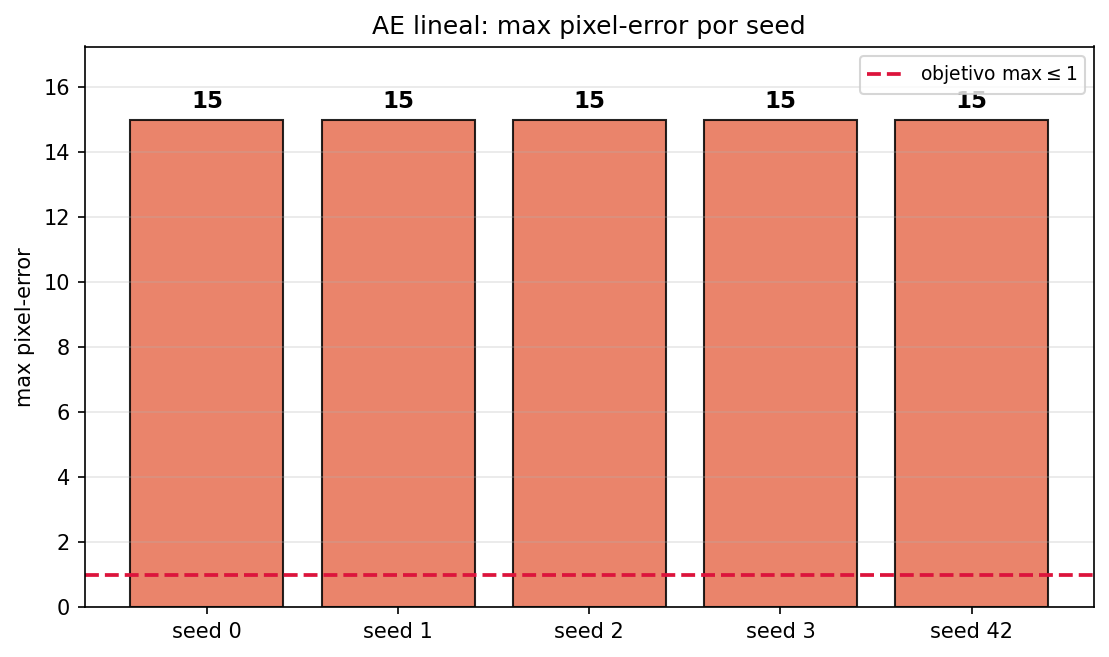
\includegraphics[width=0.72\linewidth]{exp_linear_ae.png}
\end{frame}

\begin{frame}{Una letra concreta: \texttt{'DEL'} pierde 15 de 35 pixeles}
  \centering
  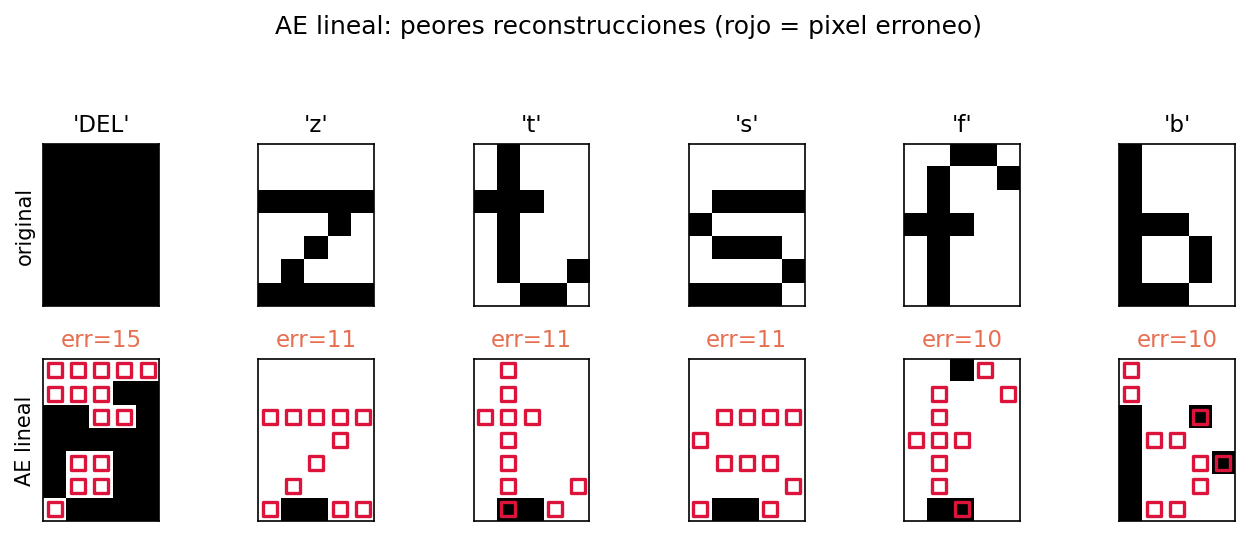
\includegraphics[width=0.95\linewidth]{exp_linear_ae_worst.png}
\end{frame}

\begin{frame}{¿Por que falla? Converge a PCA}
  \begin{columns}[T]
    \begin{column}{0.58\textwidth}
      \centering
      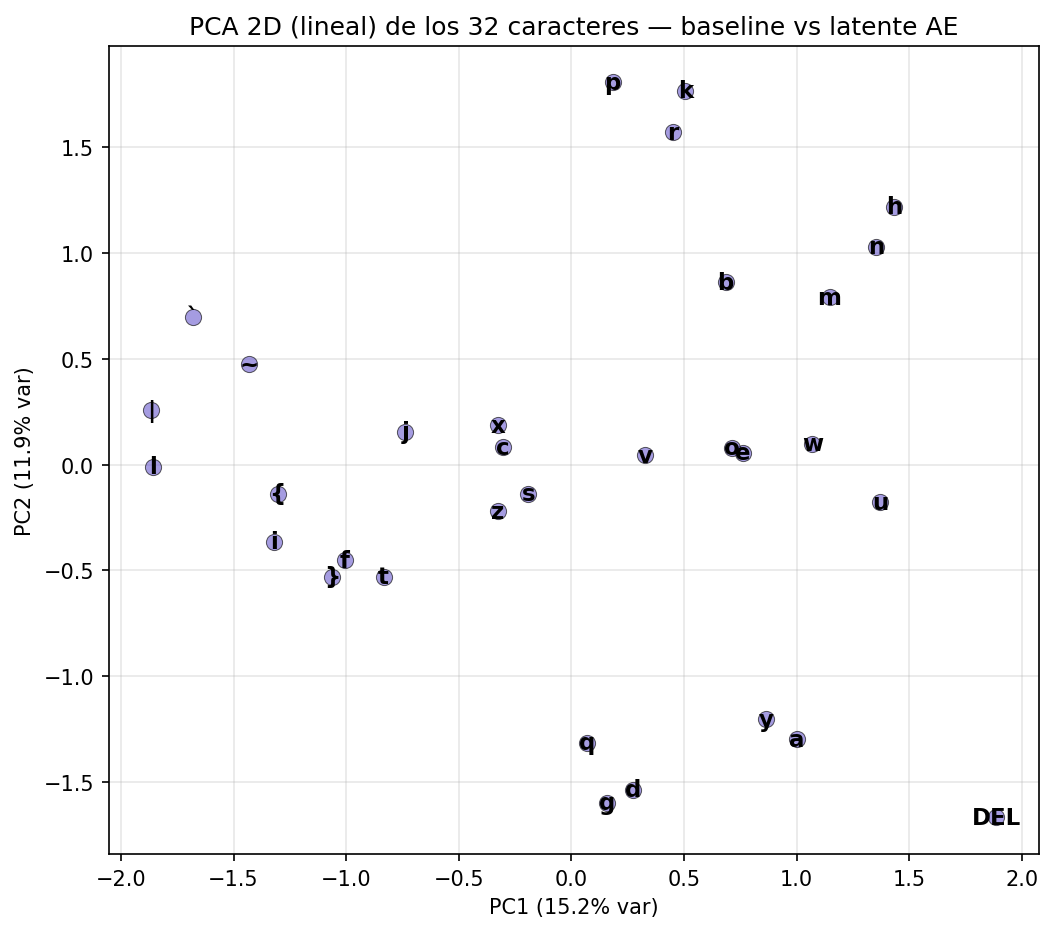
\includegraphics[width=\linewidth]{latent_scatter_pca.png}
    \end{column}
    \begin{column}{0.42\textwidth}
      \vspace{1.5em}
      \begin{itemize}
        \item Un AE \emph{lineal} \textbf{converge a PCA}.
        \item Su latente 2D retiene solo $\sim$\textbf{27\%} de la varianza
              $\Rightarrow$ no separa las 32 letras.
      \end{itemize}
    \end{column}
  \end{columns}
\end{frame}

\begin{frame}{La respuesta: no linealidad --- arquitectura base del AE}
  \begin{columns}[T]
    \begin{column}{0.52\textwidth}
      Misma idea simetrica con \textbf{cuello 2D}, pero \textbf{ocultas no lineales}:
      \[ 35 \to 60 \to 40 \to 20 \to \mathbf{2} \to 20 \to 40 \to 60 \to 35 \]
      \begin{itemize}
        \item Ocultas \textbf{tanh}; latente \textbf{lineal} (no satura);
              salida \textbf{logistica} (pixeles en $(0,1)$).
        \item Perdida \textbf{BCE}, \textbf{Adam}, full-batch, EarlyStopping.
        \item \textbf{Sin regularizacion}: queremos \emph{sobreajustar}
              (memorizar) las 32 letras.
      \end{itemize}
      \vspace{0.3em}
      {\footnotesize Esta es la \emph{configuracion base} de referencia: los
       experimentos varian \textbf{una} pieza a la vez.}
    \end{column}
    \begin{column}{0.48\textwidth}
      \centering
      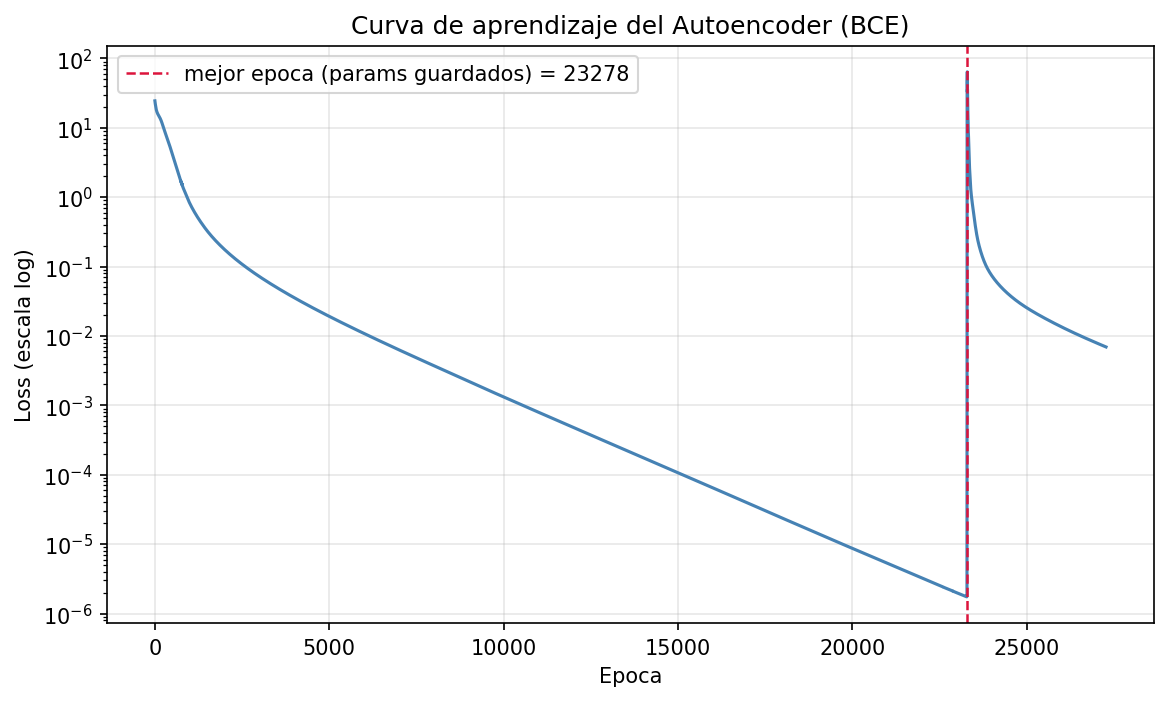
\includegraphics[width=\linewidth]{learning_curve.png}\\
      {\scriptsize Curva de loss (BCE) de la corrida principal.}
    \end{column}
  \end{columns}
\end{frame}

% ============================================================
% ESTUDIO DE OPTIMIZACION
% ============================================================

\begin{frame}[standout]
  Estudio de optimizacion

  {\normalsize Una variable a la vez, controlando el resto.}
\end{frame}

% ---- Metodologia comun (loss / activacion / arquitectura) ----

\begin{frame}{Estudio one-at-a-time: metodologia (comun a los 3 ejes)}
  \begin{columns}[T]
    \begin{column}{0.55\textwidth}
      \begin{table}\small
        \begin{tabular}{ll}
          \toprule
          Parametro & Valor \\
          \midrule
          Datos        & \texttt{font.h} ($32\times35$) \\
          Config base  & $[35,60,40,20,2,...]$, tanh, \\
                       & latente lineal, BCE, Adam $10^{-3}$ \\
          Adam $\beta_1,\beta_2,\epsilon$ & $0.9$, $0.999$, $10^{-8}$ \\
          Batch / Init & full-batch (32) / Xavier \\
          Epocas       & 6000 \\
          \textbf{Seeds}& \textbf{[0, 1, 2, 3, 42]} \\
          \midrule
          Metrica      & max pixel-error (media $\pm$ std) \\
          Criterio conv& 1a epoca con max$\le 1$ \\
          \bottomrule
        \end{tabular}
      \end{table}
    \end{column}
    \begin{column}{0.43\textwidth}
      \textbf{Pregunta}: ¿que ingredientes permiten cruzar $\le 1$ pixel, y de forma
      \emph{robusta} entre seeds?

      \vspace{0.6em}
      Variamos \textbf{una} pieza a la vez:
      \begin{enumerate}
        \item perdida (BCE / MSE)
        \item activacion oculta (tanh / relu / logistica)
        \item arquitectura (profundidad / ancho)
      \end{enumerate}
      \vspace{0.3em}
      {\footnotesize (optimizador $\times$ lr: experimento aparte.)}
    \end{column}
  \end{columns}
\end{frame}

\begin{frame}{Eje 1 --- Funcion de perdida: BCE vs MSE}
  \centering
  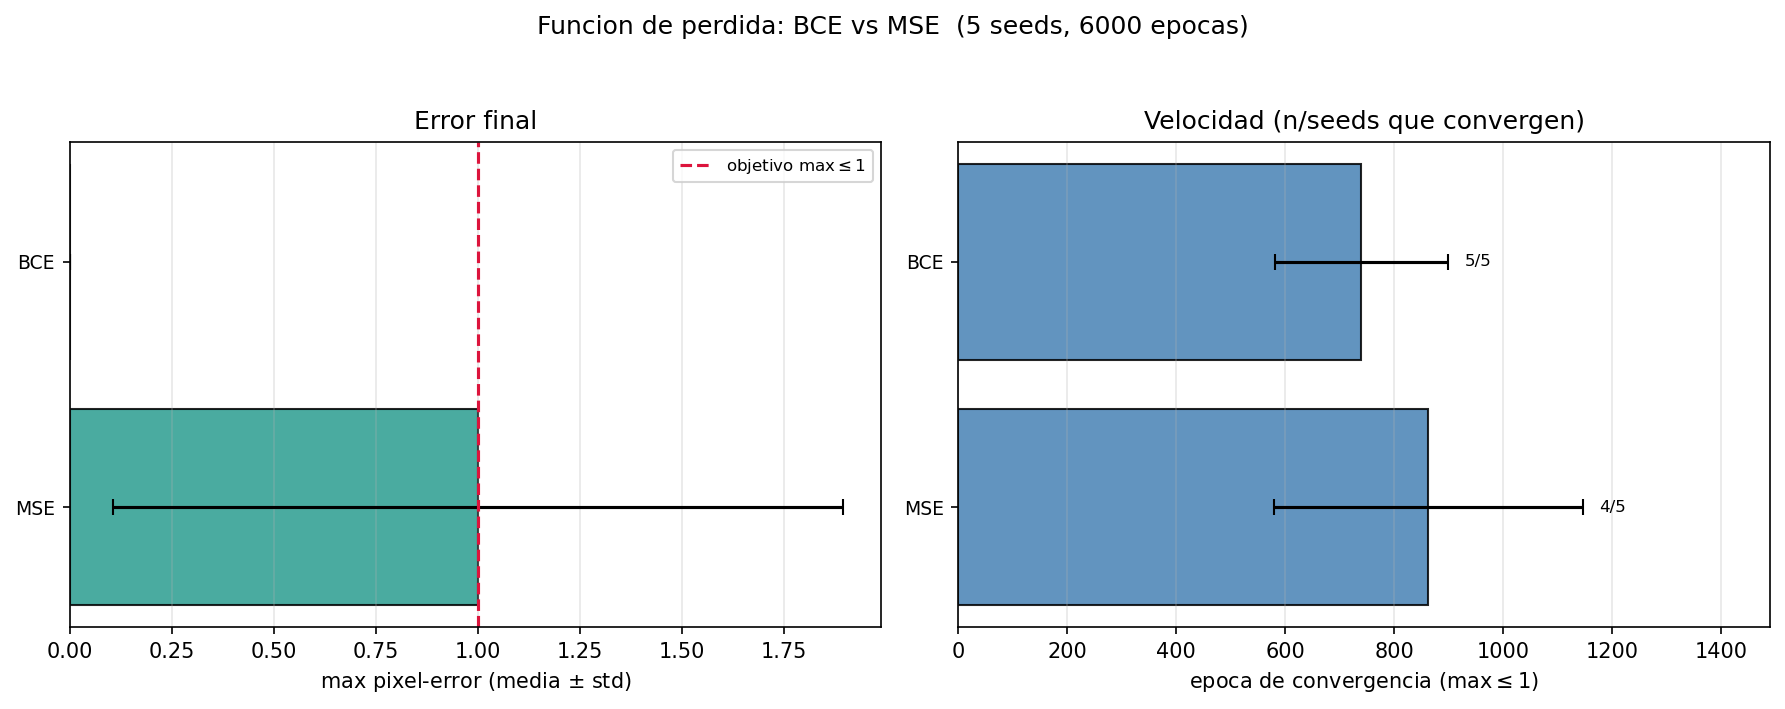
\includegraphics[width=0.9\linewidth]{exp_loss_ms.png}
  \vfill
  {\footnotesize \textbf{BCE} 5/5 vs \textbf{MSE} \emph{borderline} (4/5).
   \textbf{Fijamos BCE}.}
\end{frame}

\begin{frame}{Eje 2 --- Activacion oculta: tanh / relu / logistica}
  \centering
  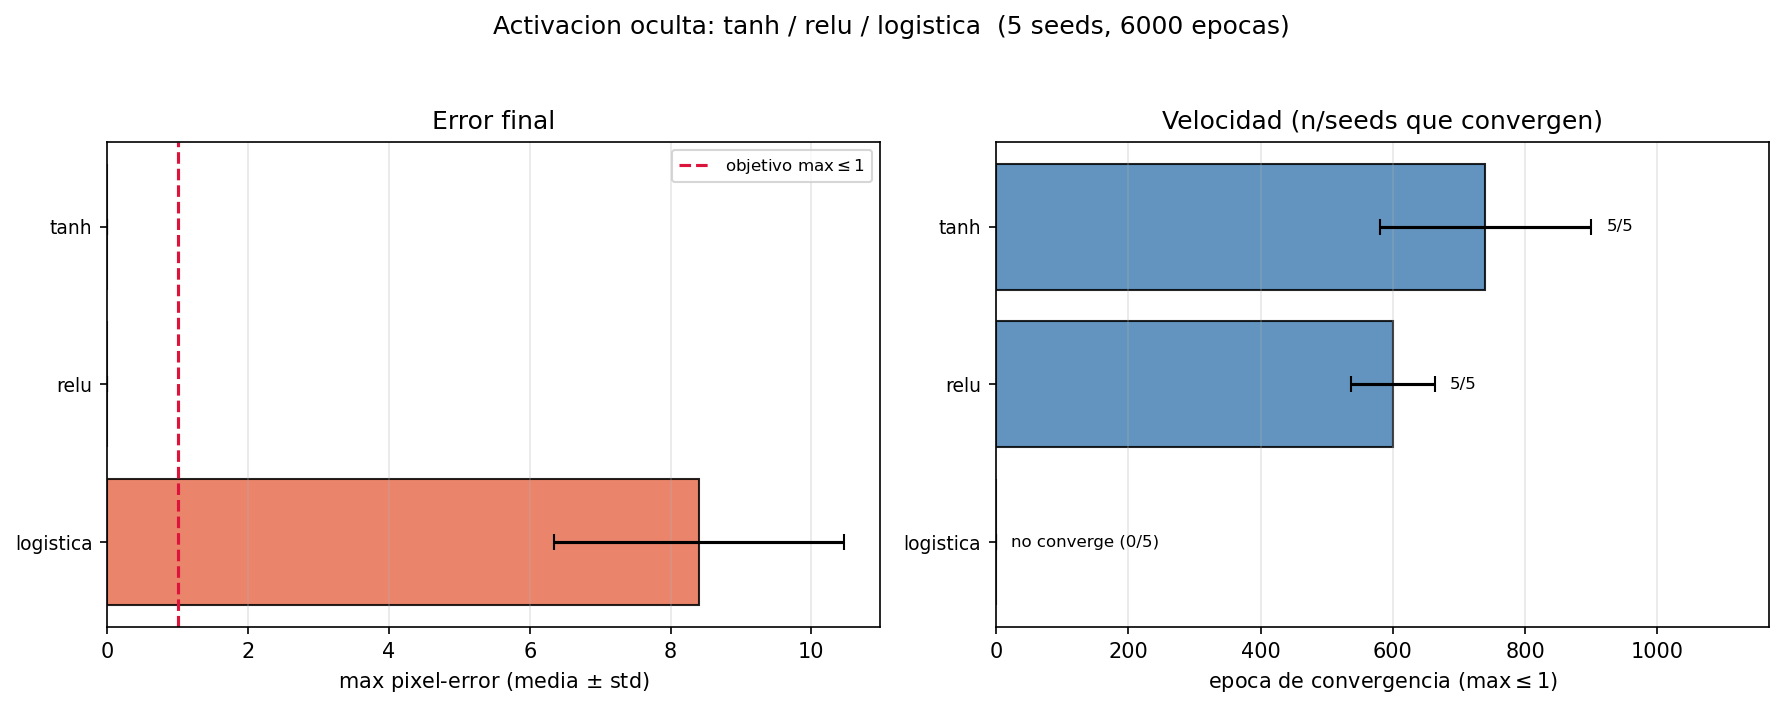
\includegraphics[width=0.9\linewidth]{exp_activation_ms.png}
  \vfill
  {\footnotesize \textbf{tanh}/\textbf{relu} 5/5; \textbf{logistica} 0/5 (satura el
   gradiente). \textbf{Fijamos tanh}.}
\end{frame}

\begin{frame}{Eje 3 --- Arquitectura: profundidad / ancho}
  \centering
  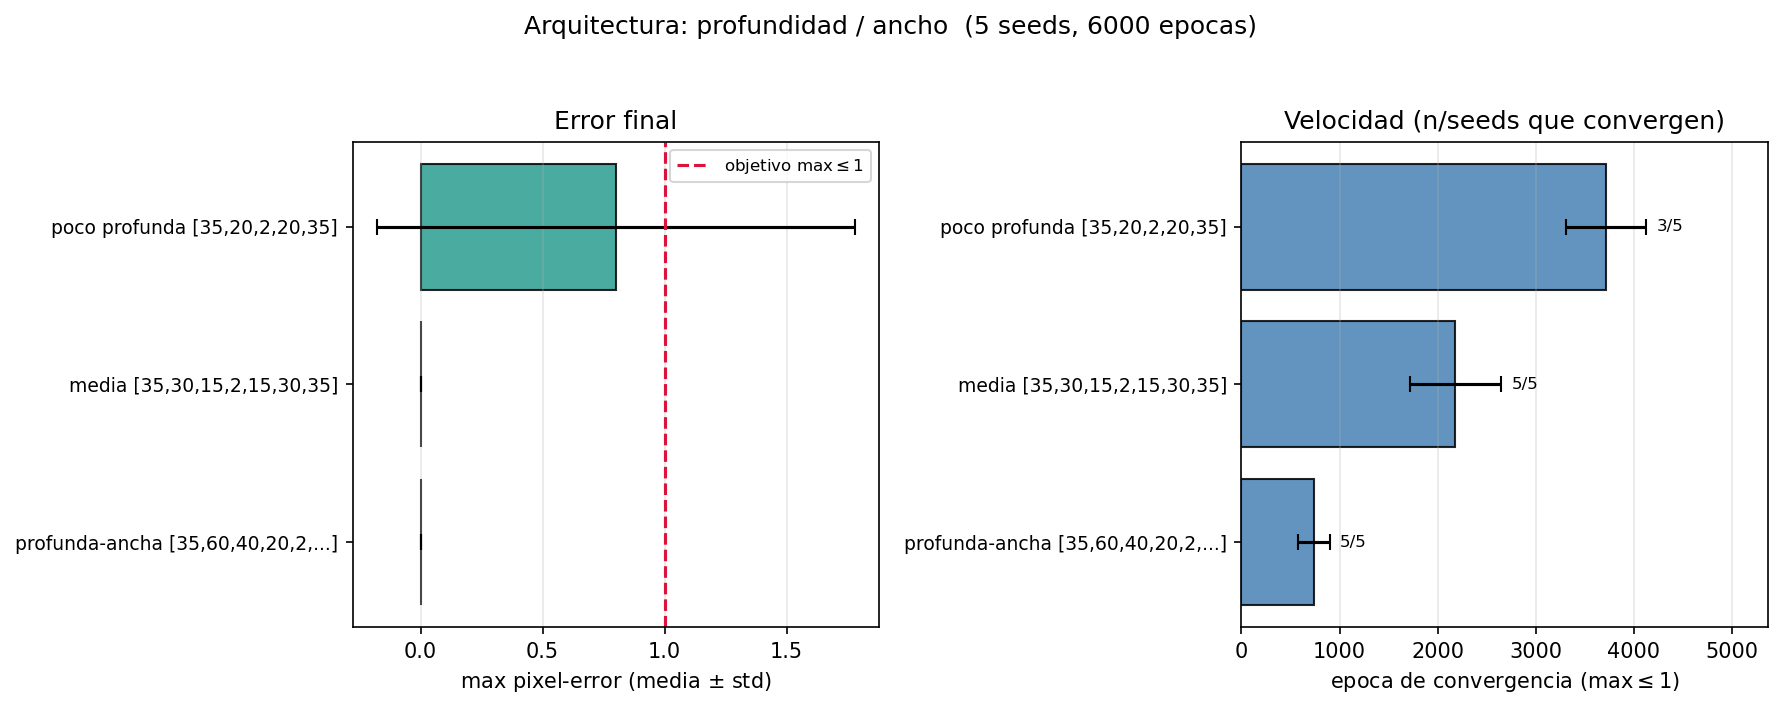
\includegraphics[width=0.9\linewidth]{exp_architecture_ms.png}
  \vfill
  {\footnotesize \textbf{poco profunda} inestable (3/5); mas profundidad/ancho
   $\Rightarrow$ confiable. \textbf{Fijamos la profunda-ancha} (5/5).}
\end{frame}

% ---- EXP 4: optimizador x lr (con censura) ----

\begin{frame}{Eje 4 --- Optimizador $\times$ learning rate: parametros}
  \begin{columns}[T]
    \begin{column}{0.54\textwidth}
      \begin{table}\small
        \begin{tabular}{ll}
          \toprule
          Parametro & Valor \\
          \midrule
          Datos          & \texttt{font.h} ($32\times35$) \\
          Config base    & profunda-ancha, tanh, BCE \\
          Batch / Init   & full-batch (32) / Xavier \\
          \midrule
          \textit{Variable} & optimizador $\times$ lr \\
          optimizador    & GD / Momentum(0.9) / Adam \\
          Adam $\beta_1,\beta_2,\epsilon$ & $0.9$, $0.999$, $10^{-8}$ \\
          lr             & $10^{-4}$ a $10^{-2}$ (5 valores) \\
          \midrule
          Protocolo      & \textbf{5 seeds $\times$ 30000 ep} \\
          \bottomrule
        \end{tabular}
      \end{table}
    \end{column}
    \begin{column}{0.44\textwidth}
      \textbf{Pregunta}:
      \begin{itemize}
        \item ¿el lr optimo \emph{depende} del optimizador?, ¿es Adam robusto al lr?
      \end{itemize}
    \end{column}
  \end{columns}
\end{frame}

\begin{frame}{Eje 4 --- Optimizador $\times$ learning rate (5 seeds $\times$ 30000 ep)}
  \centering
  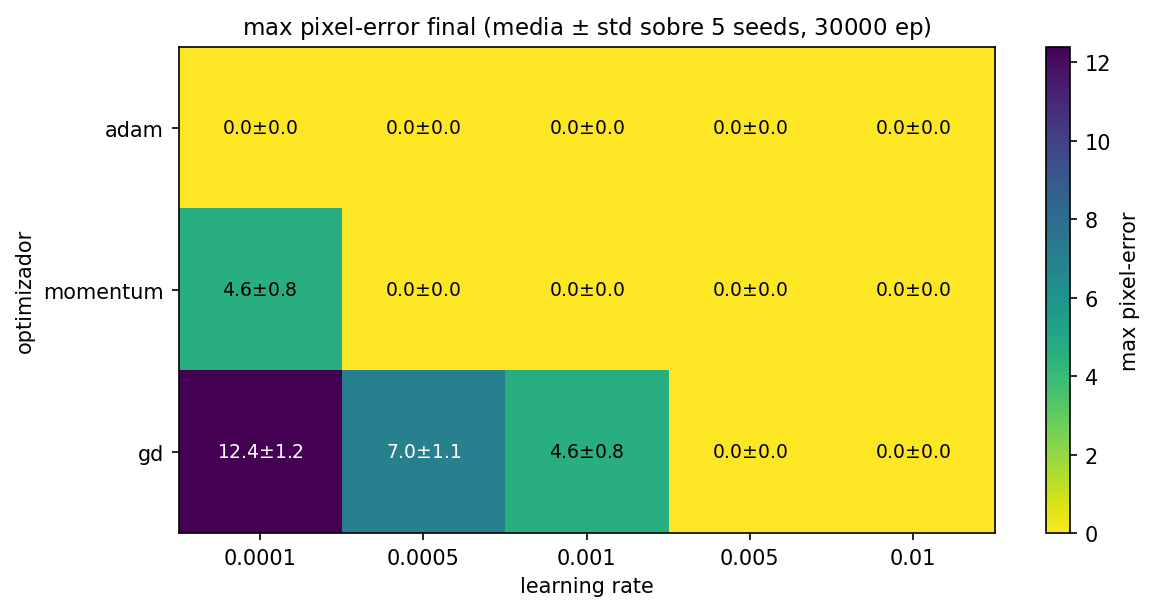
\includegraphics[width=0.78\linewidth]{exp_grid_full_maxpix.png}
  \vfill
  {\footnotesize \textbf{Adam}: max$=0$ en \emph{todo} el rango de lr (robusto).
   GD y Momentum solo con lr altos. \textbf{Fijamos Adam}.}
\end{frame}

% ============================================================
% RESULTADOS
% ============================================================

\section{Resultados}

\begin{frame}{Objetivo $\le 1$ pixel: CUMPLIDO}
  \begin{columns}[T]
    \begin{column}{0.50\textwidth}
      \begin{table}\scriptsize
        \begin{tabular}{ll}
          \toprule
          \multicolumn{2}{l}{\textbf{Configuracion del modelo final}} \\
          \midrule
          Arquitectura  & $[35,60,40,20,\mathbf{2},20,40,60,35]$ \\
          Activaciones  & tanh / latente lineal / logistica \\
          Perdida / Opt & BCE / Adam (lr $=10^{-3}$) \\
          Adam $\beta_1,\beta_2,\epsilon$ & $0.9$, $0.999$, $10^{-8}$ \\
          Init / Epocas & Xavier / 30000 \\
          Early stopping & patience $4000$, min$\Delta=10^{-7}$ \\
          Batch / Seed  & full-batch (32) / 0 \\
          \bottomrule
        \end{tabular}
      \end{table}
      \begin{table}\scriptsize
        \begin{tabular}{lr}
          \toprule
          Metrica & Valor \\
          \midrule
          max pixel-error      & \textbf{0} \\
          letras exactas       & \textbf{32/32} \\
          BCE final (mejor ep) & $1.74\times10^{-6}$ \\
          \bottomrule
        \end{tabular}
      \end{table}
      {\scriptsize Cumplido \textbf{con margen} (max$=0$). Las 5 seeds llegan a
       max$=0$; \texttt{model.npz} reproduce el resultado.}
    \end{column}
    \begin{column}{0.50\textwidth}
      \centering
      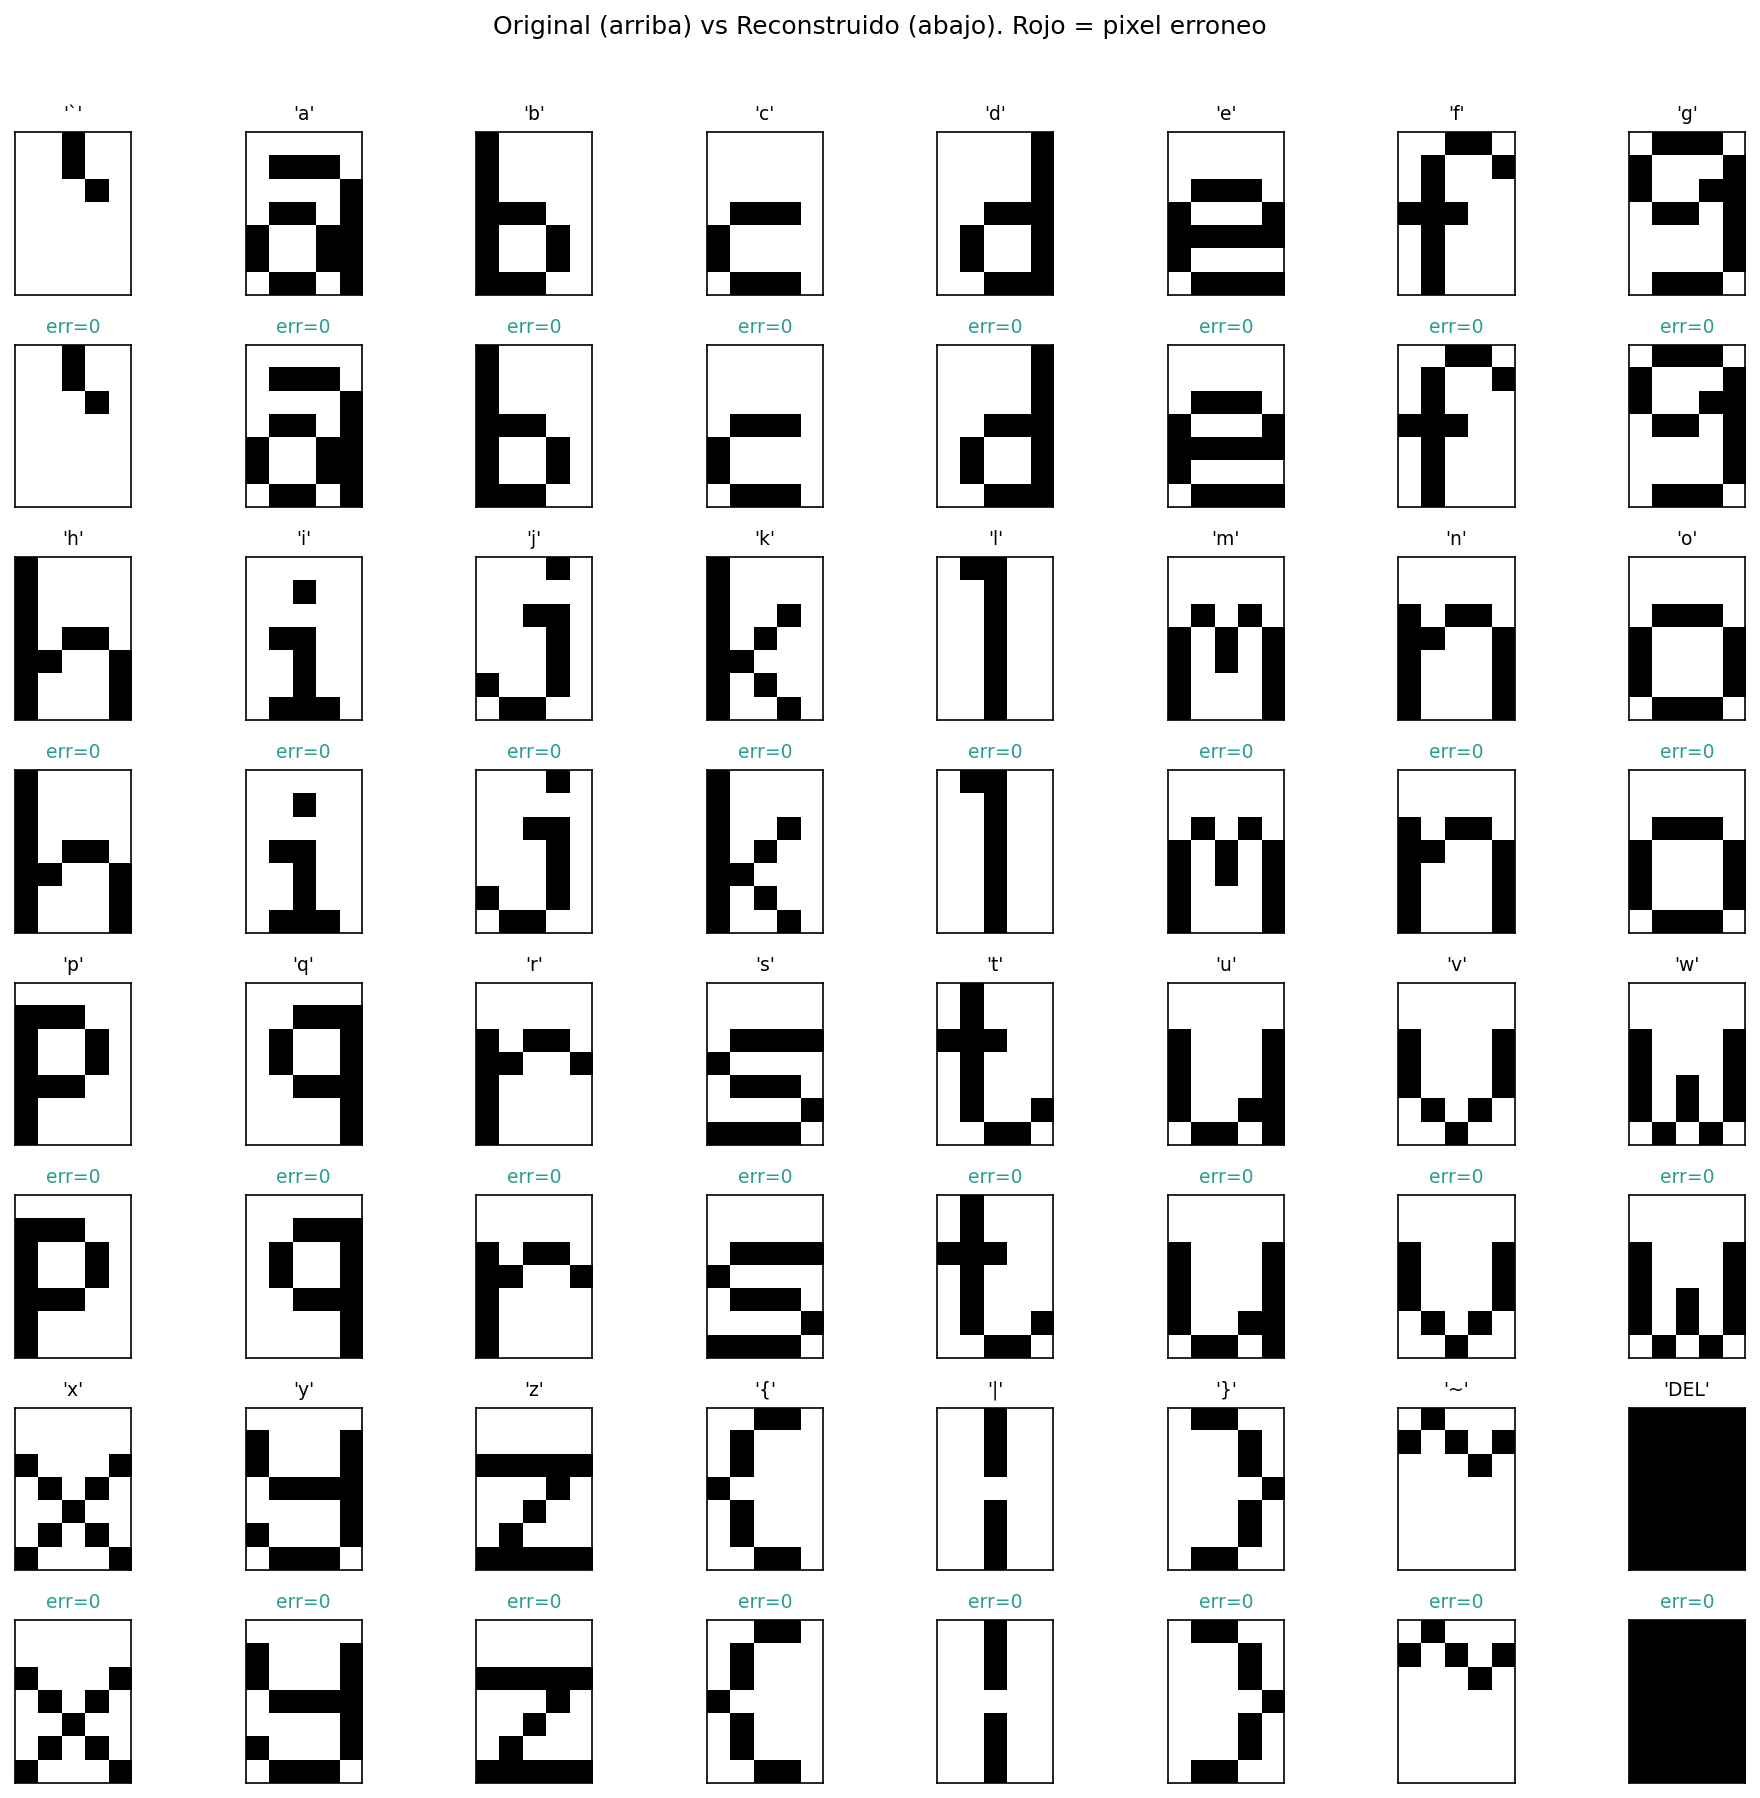
\includegraphics[width=\linewidth]{reconstruction_grid.png}\\
      {\scriptsize Original (arriba) vs reconstruccion (abajo); rojo = pixel erroneo.}
    \end{column}
  \end{columns}
\end{frame}

\begin{frame}{Espacio latente 2D del AE}
  \begin{columns}[T]
    \begin{column}{0.52\textwidth}
      \centering
      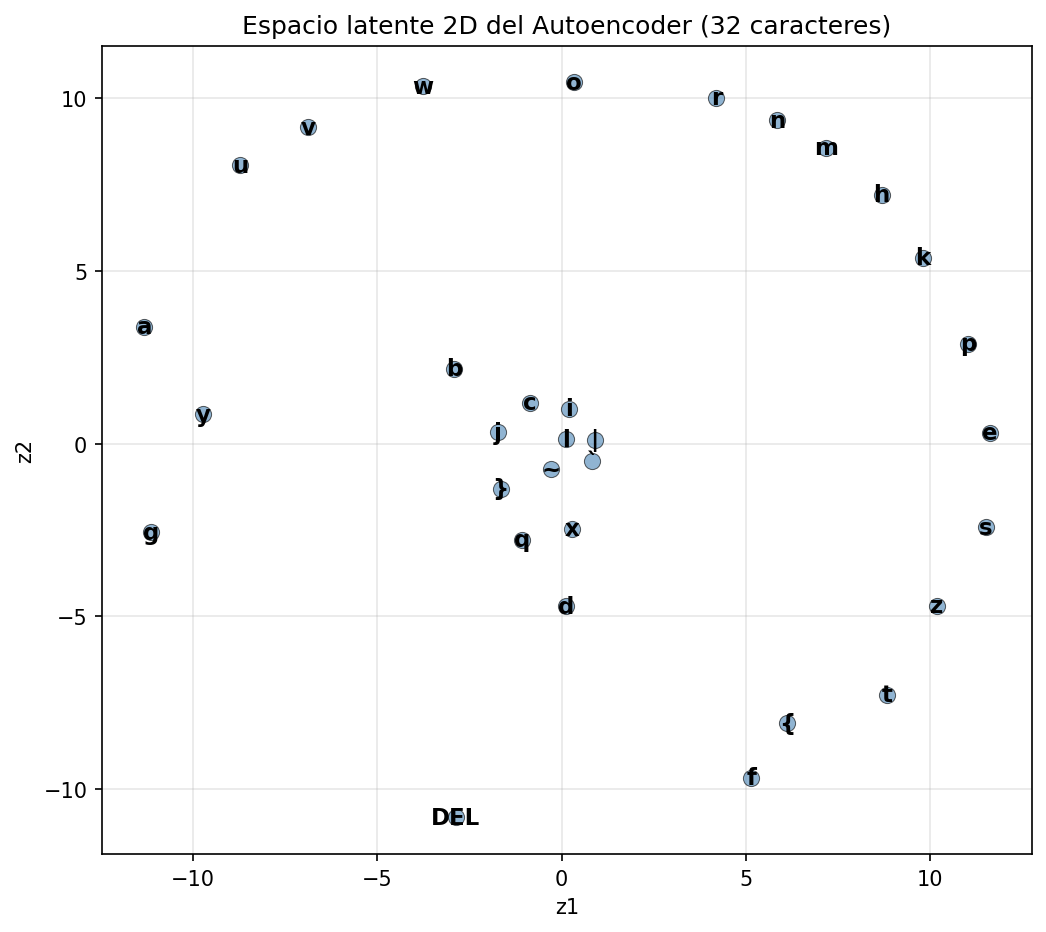
\includegraphics[width=\linewidth]{latent_scatter.png}\\
      {\scriptsize Latente 2D del AE no lineal (32 letras).}
    \end{column}
    \begin{column}{0.48\textwidth}
      \begin{itemize}
        \item El AE \emph{no lineal} ubica las 32 letras en posiciones bien
              separadas del plano 2D.
        \item Mismo cuello 2D que el PCA, pero aca reconstruye \textbf{perfecto}
              (vs 27\% de varianza del PCA lineal).
      \end{itemize}
    \end{column}
  \end{columns}
\end{frame}

\begin{frame}{Generar una letra nueva (interpolacion)}
  \centering
  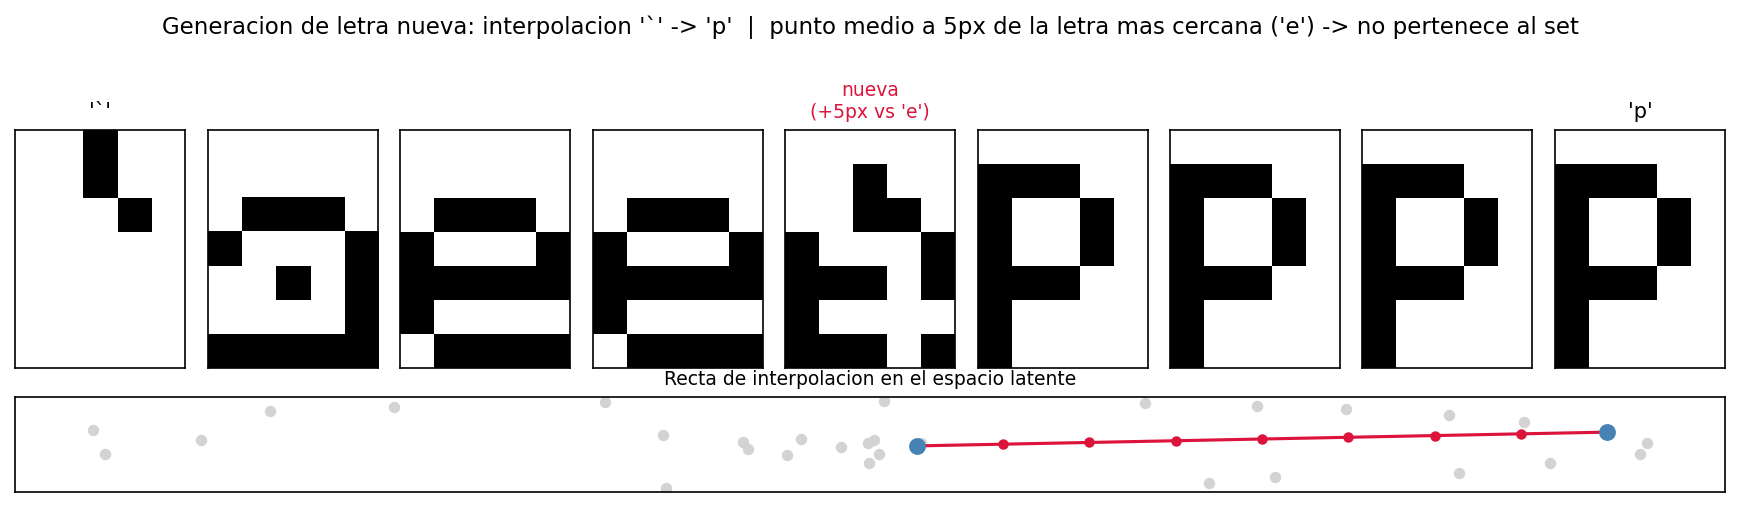
\includegraphics[width=0.98\linewidth]{new_letter_generation.png}
  \vfill
\end{frame}

\begin{frame}{El latente del AE no es generativo}
  \begin{columns}[T]
    \begin{column}{0.58\textwidth}
      \centering
      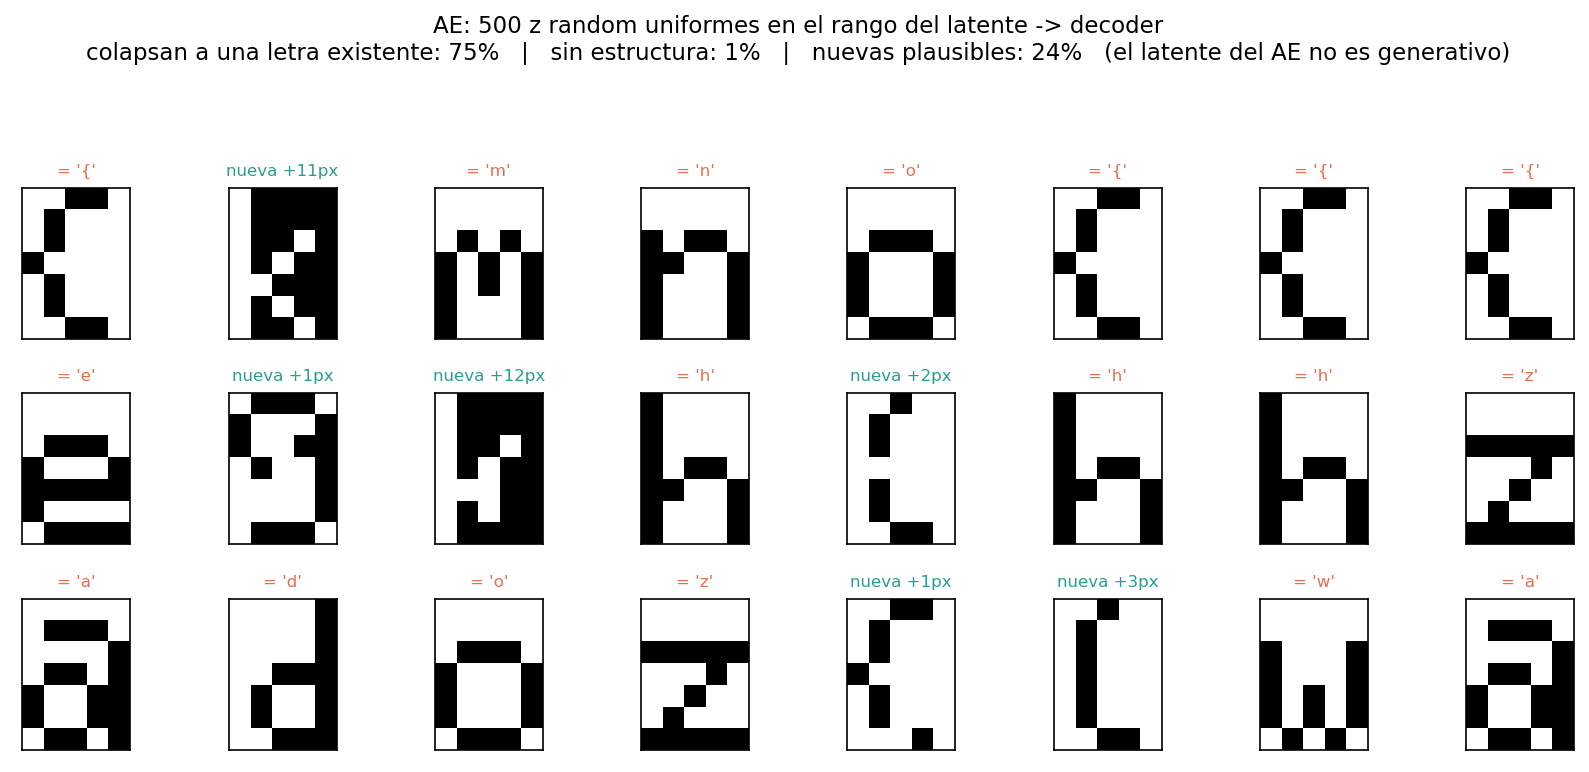
\includegraphics[width=\linewidth]{random_latent_sampling.png}
    \end{column}
    \begin{column}{0.42\textwidth}
      \begin{itemize}
        \item Muestreamos 500 puntos $z$ \emph{al azar} en el rango del latente
              y decodificamos.
        \item \textbf{75\%} colapsa a una letra existente; \textbf{24\%} son
              "nuevas plausibles".
        \item El \textbf{1\%} restante es un patron \emph{sin estructura}, que no
              podria considerarse una nueva letra:
      \end{itemize}
      \vspace{0.2em}
      \centering
      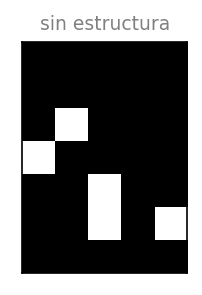
\includegraphics[height=0.30\textheight]{random_latent_sampling_noise_example.png}
    \end{column}
  \end{columns}
\end{frame}

% ============================================================
% DENOISING AUTOENCODER (EJ1.b)
% ============================================================

\section{Denoising Autoencoder}

\begin{frame}{Planteo del DAE --- setup y ruido}
  \begin{columns}[T]
    \begin{column}{0.56\textwidth}
      \begin{table}\small
        \begin{tabular}{ll}
          \toprule
          Parametro & Valor \\
          \midrule
          Datos        & \texttt{font.h} ($32\times35$) \\
          Tarea        & entrada ruidosa $\to$ target limpio \\
          Augmentation & online (ruido nuevo cada epoca) \\
          Arquitectura & $[35,60,40,20,8,20,40,60,35]$ \\
          Activaciones & tanh (oculta), logistica (salida) \\
                       & cuello \emph{lineal} (identidad) \\
          Loss / Opt   & BCE / Adam $10^{-3}$ \\
          Epocas / Batch / Init & 12000 / full-batch / Xavier \\
          Ruido train  & salt\&pepper $p=0.10$ \\
          \textbf{Seeds} & \textbf{[0, 1, 2, 3, 42]} \\
          \bottomrule
        \end{tabular}
      \end{table}
    \end{column}
    \begin{column}{0.44\textwidth}
      \textbf{Modelos de ruido} (barrido de evaluacion):
      \begin{itemize}
        \item \textbf{salt\&pepper}: invierte cada pixel con prob. $p$.
        \item \textbf{gaussian}: $x + \mathcal{N}(0,\sigma^2)$, clip a $[0,1]$.
        \item \textbf{masking}: pone a 0 una fraccion de pixeles.
      \end{itemize}
      \vspace{0.3em}
      {\footnotesize Se entrena solo con salt\&pepper; gaussian y masking
       miden \emph{generalizacion} a ruido no visto.}
    \end{column}
  \end{columns}
\end{frame}

\begin{frame}{Estudio 1 --- ¿Que cuello? 2D vs 4D vs 8D}
  \centering
  {\scriptsize\color{gray} Varia: tamano del cuello (resto fijo: ver planteo).
   5 seeds [0,1,2,3,42].}
  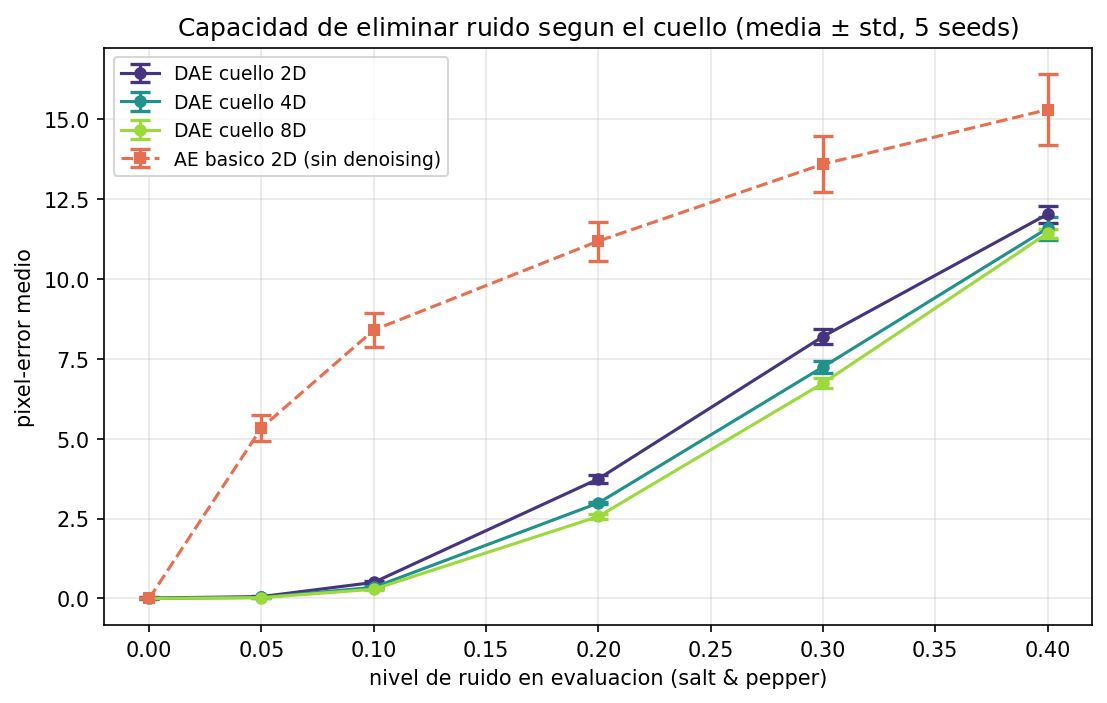
\includegraphics[width=0.72\linewidth]{dae_bottleneck_curves.png}
  \vfill
  {\footnotesize \textbf{2D queda corto} (31.8/32 limpio); \textbf{4D} satura y
   \textbf{8D} es mejor por poco. Barras $=$ std de 5 seeds.}
\end{frame}

\begin{frame}{Estudio 2 --- nivel de ruido en train: parametros}
  \begin{columns}[T]
    \begin{column}{0.55\textwidth}
      \begin{table}\small
        \begin{tabular}{ll}
          \toprule
          Parametro & Valor \\
          \midrule
          Datos         & \texttt{font.h} ($32\times35$) \\
          Config base   & DAE \textbf{cuello 8D} (Estudio 1), \\
                        & lineal, tanh, BCE, Adam $10^{-3}$ \\
          Entrenamiento & salt\&pepper online, target limpio \\
          Batch / Init  & full-batch (32) / Xavier \\
          Epocas        & 12000 \\
          \textbf{Seeds}& \textbf{[0, 1, 2, 3, 42]} \\
          Metrica       & pixel-error medio (32 letras \\
                        & $\times$ 20 realizaciones) \\
          \bottomrule
        \end{tabular}
      \end{table}
    \end{column}
    \begin{column}{0.44\textwidth}
      \textit{Variable}: \textbf{nivel de ruido en train}
      $p \in \{0.05, 0.10, 0.20, 0.30\}$ (un DAE por nivel).

      \vspace{0.6em}
      \textbf{Pregunta}: ¿cuanto ruido conviene en train para generalizar a
      distintos niveles?

      \vspace{0.4em}
      {\footnotesize Eval: barriendo el ruido $0\to0.40$; \textbf{media $\pm$ std}
       sobre las 5 seeds.}
    \end{column}
  \end{columns}
\end{frame}

\begin{frame}{Estudio 2 --- ¿Cuanto ruido conviene en train?}
  \centering
  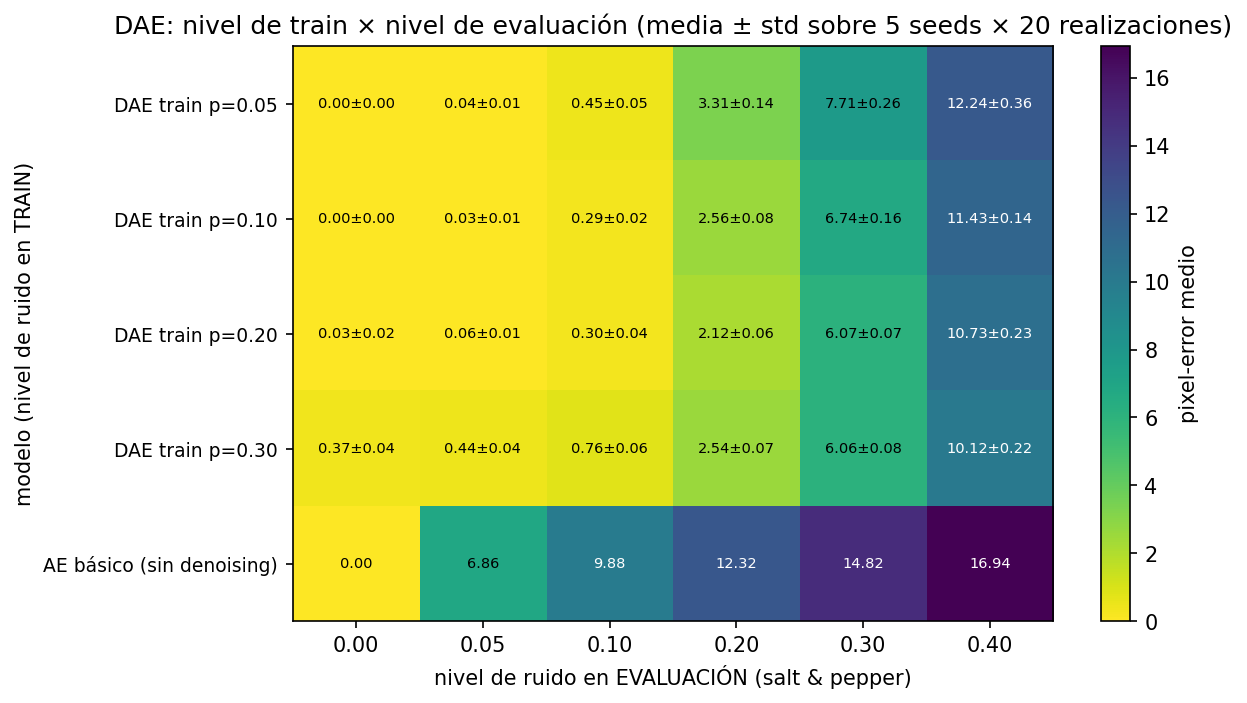
\includegraphics[width=0.78\linewidth]{exp_train_levels_heatmap.png}
  \vfill
  {\footnotesize \textbf{Sweet spot $p\approx0.10$--$0.20$}: $p=0.05$ generaliza
   mal a ruido fuerte; $p=0.30$ ya degrada el limpio.}
\end{frame}

\begin{frame}{Estudio 3 --- activacion del cuello: parametros}
  \begin{columns}[T]
    \begin{column}{0.55\textwidth}
      \begin{table}\small
        \begin{tabular}{ll}
          \toprule
          Parametro & Valor \\
          \midrule
          Datos         & \texttt{font.h} ($32\times35$) \\
          Config base   & DAE \textbf{cuello 8D} (Estudios 1--2), \\
                        & tanh oculta, BCE, Adam $10^{-3}$ \\
          Entrenamiento & salt\&pepper online $p{=}0.10$, \\
                        & target limpio \\
          Batch / Init  & full-batch (32) / Xavier \\
          Epocas        & 12000 \\
          \textbf{Seeds}& \textbf{[0, 1, 2, 3, 42]} \\
          Metrica       & pixel-error medio (32 letras \\
                        & $\times$ 20 realizaciones) \\
          \bottomrule
        \end{tabular}
      \end{table}
    \end{column}
    \begin{column}{0.44\textwidth}
      \textit{Variable}: \textbf{activacion del cuello}
      $\in \{$identidad, tanh$\}$.

      \vspace{0.6em}
      \textbf{Pregunta}: ¿la activacion del latente cambia el denoising?
      (en 1a el cuello era lineal).

      \vspace{0.4em}
      {\footnotesize Eval: barriendo el ruido $0\to0.40$; \textbf{media $\pm$ std}
       sobre las 5 seeds.}
    \end{column}
  \end{columns}
\end{frame}

\begin{frame}{Estudio 3 --- ¿Importa la activacion del cuello?}
  \centering
  {\scriptsize\color{gray} Varia: activacion del cuello, identidad vs tanh
   (resto fijo: ver parametros). 5 seeds.}
  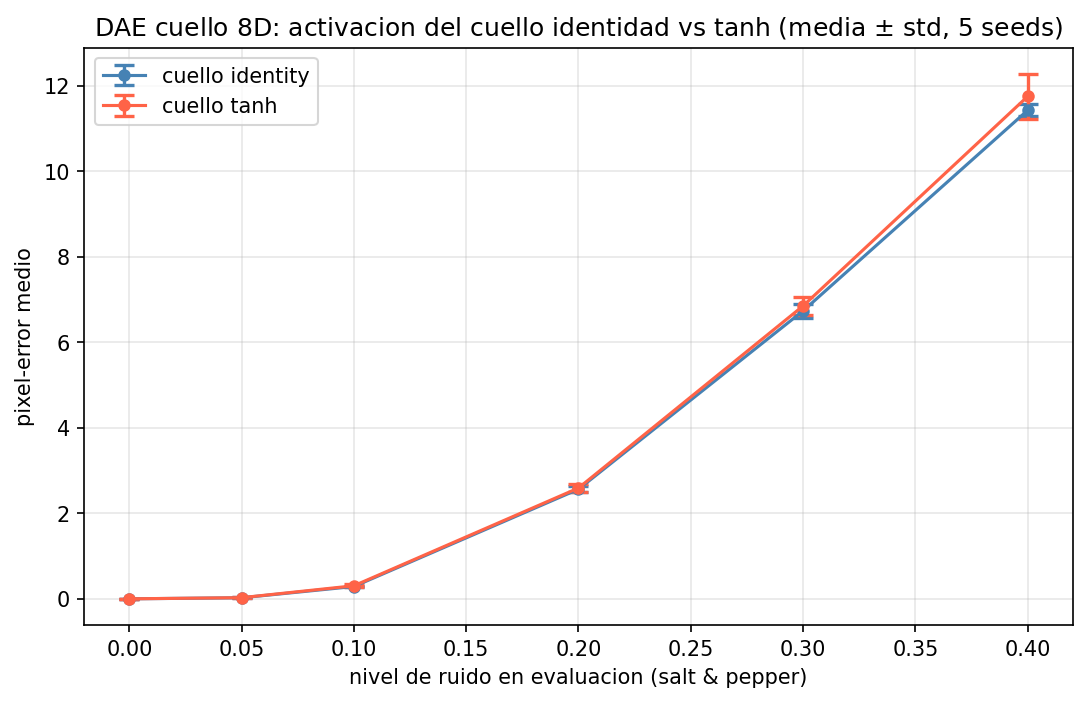
\includegraphics[width=0.72\linewidth]{dae_bnactivation_curves.png}
  \vfill
  {\footnotesize \textbf{Empate}: ambas reconstruyen el limpio (32/32) y dan el
   mismo denoising dentro del std. Identidad es igual o levemente mejor y mas
   estable $\Rightarrow$ \textbf{usamos identidad} (coherente con 1a).}
\end{frame}

\begin{frame}{Capacidad de denoising (cualitativo)}
  \centering
  {\scriptsize\color{gray} DAE final: cuello 8D, entrenado con salt\&pepper $p=0.10$.}
  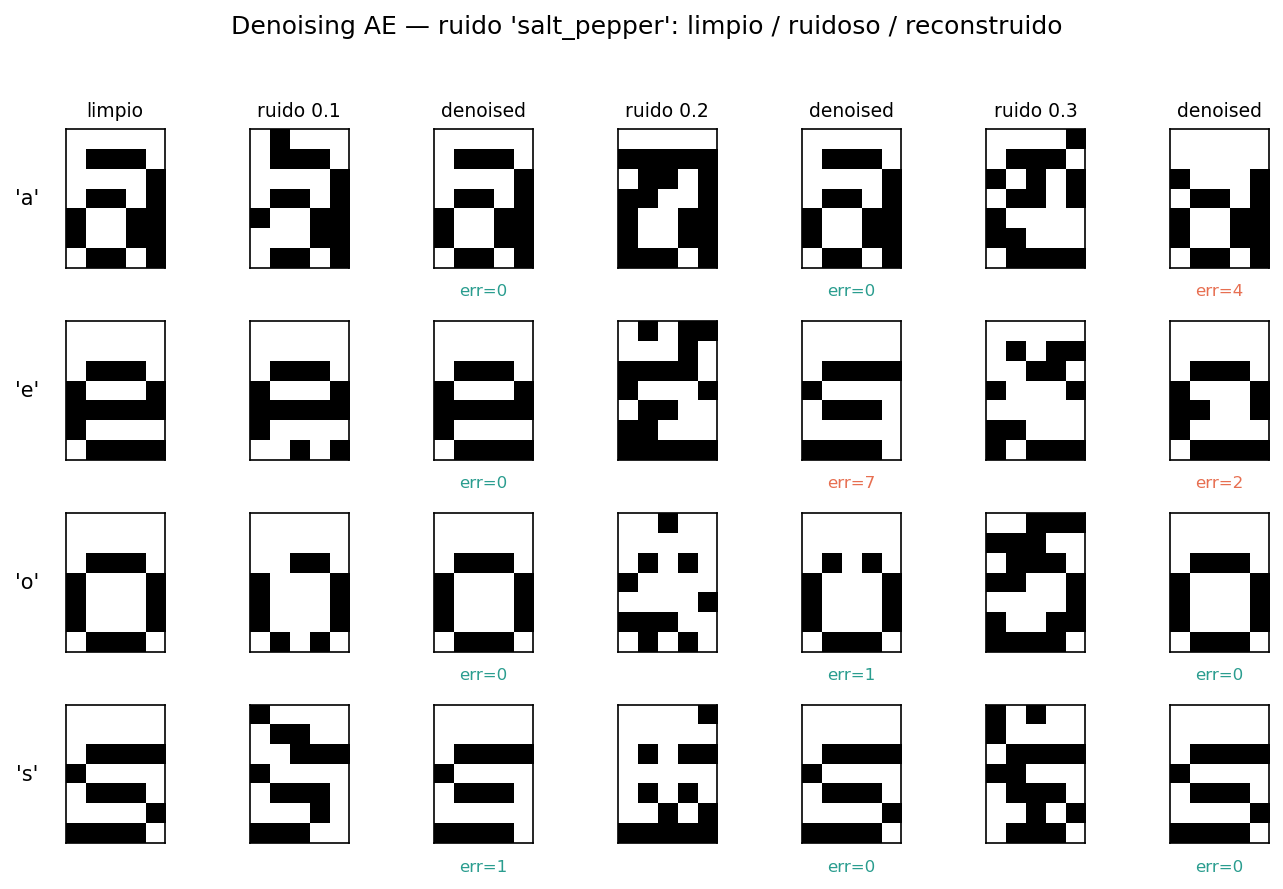
\includegraphics[width=0.75\linewidth]{noise_examples.png}
  \vfill
  {\footnotesize Limpia bien hasta $p\approx0.2$--$0.3$ (\texttt{err=0});
   a ruido fuerte empieza a fallar en letras densas.}
\end{frame}

\begin{frame}{Robustez --- DAE vs AE basico: parametros}
  \begin{columns}[T]
    \begin{column}{0.55\textwidth}
      \begin{table}\small
        \begin{tabular}{ll}
          \toprule
          Parametro & Valor \\
          \midrule
          Datos        & \texttt{font.h} ($32\times35$) \\
          DAE          & cuello \textbf{8D} lineal, train \\
                       & salt\&pepper $p=0.10$ (online) \\
          AE basico    & cuello \textbf{2D} lineal, \\
                       & \emph{sin} ruido (input=target) \\
          Loss / Opt   & BCE / Adam $10^{-3}$ \\
          Epocas       & DAE 12000 / basico 30000 \\
          \textbf{Seeds}& \textbf{[0, 1, 2, 3, 42]} \\
          Metrica      & pixel-error medio (32 letras \\
                       & $\times$ 20 realizaciones) \\
          \bottomrule
        \end{tabular}
      \end{table}
    \end{column}
    \begin{column}{0.44\textwidth}
      \textit{Comparacion}: \textbf{3 tipos de ruido} (salt\&pepper, gaussian,
      masking), barriendo el nivel $0\to0.40$.

      \vspace{0.6em}
      \textbf{Pregunta}: ¿el denoising es un efecto \emph{aprendido}?
    \end{column}
  \end{columns}
\end{frame}

\begin{frame}{Robustez al ruido: DAE vs AE basico}
  \centering
  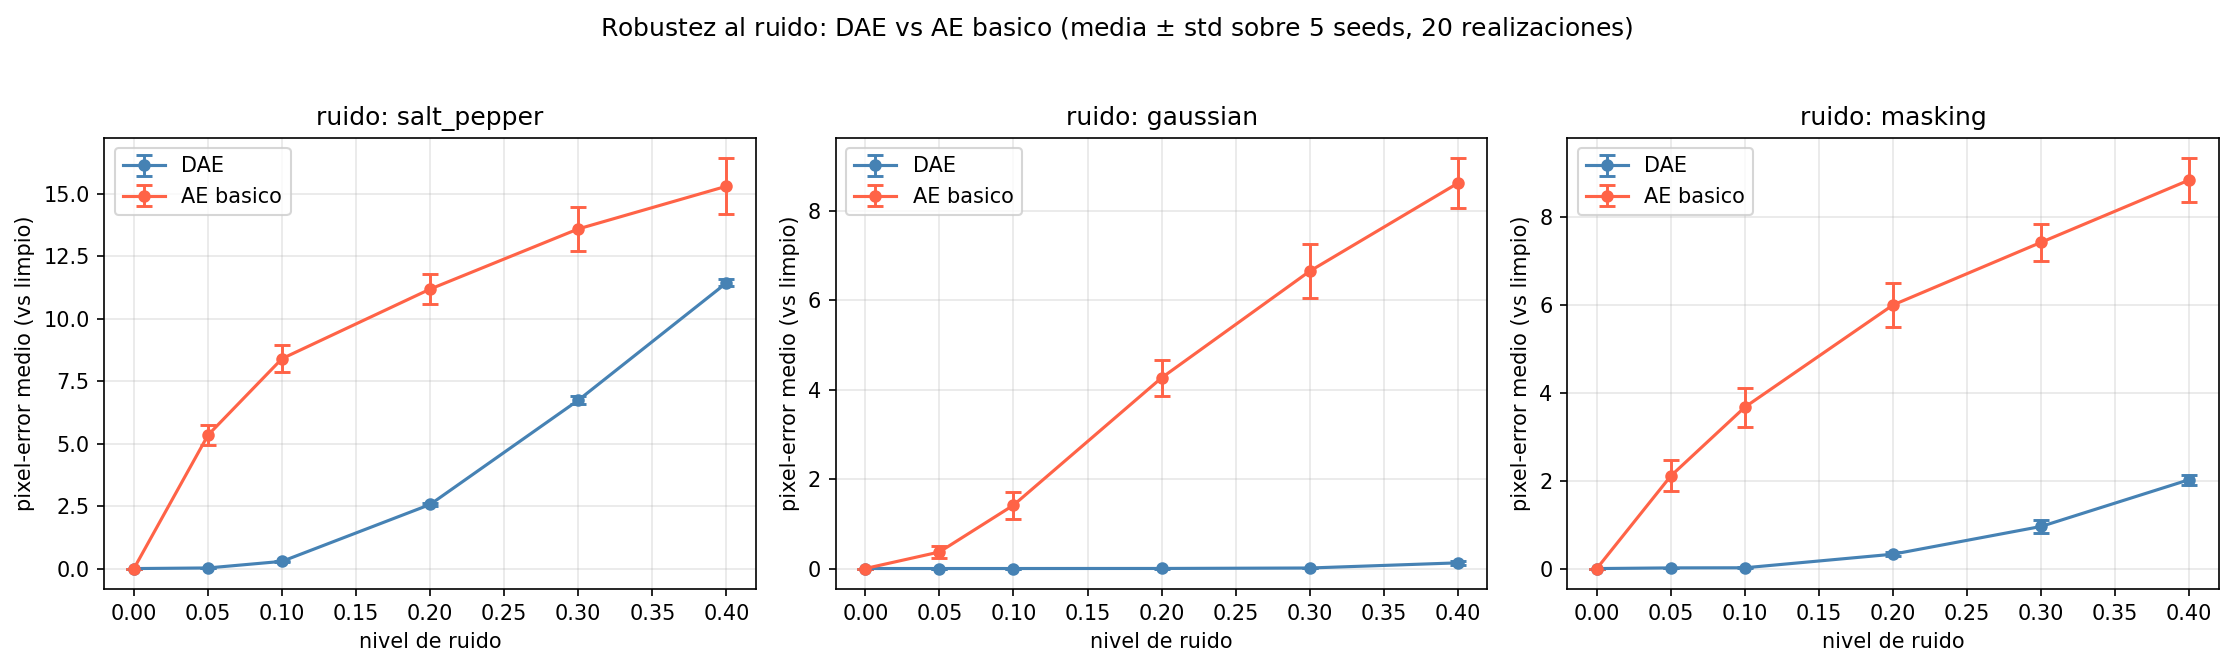
\includegraphics[width=0.96\linewidth]{dae_robustness_sweep.png}
  \vfill
  {\footnotesize El DAE queda \textbf{muy por debajo} en error en los 3 ruidos,
   incluso en \emph{gaussian} y \emph{masking} que \textbf{no vio en train}.}
\end{frame}

% ============================================================
% CONCLUSIONES
% ============================================================

\section{Conclusiones}

\begin{frame}{Conclusiones}
  \begin{itemize}\setlength\itemsep{6pt}
    \item Un AE no lineal con cuello \textbf{2D} memoriza las 32 letras con \textbf{0 píxeles de error},
          muy por encima del baseline PCA 2D.
    \item \textbf{Receta robusta}: BCE + tanh + Adam funciona bien y es insensible al lr.
    \item El \textbf{DAE} limpia salt\&pepper hasta $p\approx0.2$--$0.3$ y generaliza a ruidos
          no vistos en train (gaussian, masking).
    \item Cuello \textbf{8D lineal} es óptimo para denoising; el nivel de ruido de train tiene
          un sweet spot en $p\approx0.10$--$0.20$.
    \item \textbf{Límite del AE}: el espacio latente \textbf{no tiene estructura}; muestrear
          puntos arbitrarios no genera letras válidas. $\Rightarrow$ necesitamos un espacio
          latente organizado.
  \end{itemize}
\end{frame}

\end{document}
